% INSE 6450 - Milestone 4 - EV Plug Occupancy Forecaster
% Yellow boxes (\run / \fillin) must be filled in before submitting.
% \run = number produced by the champion-challenger simulation (not run yet).
% Compile with pdflatex (run twice for references).
\documentclass[11pt,letterpaper]{article}
\usepackage[margin=0.9in]{geometry}
\usepackage[T1]{fontenc}
\usepackage[utf8]{inputenc}
\usepackage{amsmath}
\usepackage{booktabs}
\usepackage{tabularx}
\usepackage{enumitem}
\usepackage[table]{xcolor}
\usepackage{caption}
\usepackage{graphicx}
\usepackage{float}
\usepackage{tikz}
\usetikzlibrary{positioning,arrows.meta,fit,backgrounds}
\usepackage[colorlinks=true,linkcolor=blue!50!black,urlcolor=blue!50!black,citecolor=blue!50!black]{hyperref}

\usepackage{algorithm}
\usepackage{algpseudocode}

\setlength{\parindent}{0pt}
\setlength{\parskip}{5pt}
\captionsetup{font=small,labelfont=bf}
\setlist{itemsep=1pt,topsep=2pt}

\newcommand{\run}{\colorbox{yellow}{\footnotesize RUN}}
\newcommand{\fillin}[1]{\colorbox{yellow}{#1}}
\newcolumntype{Y}{>{\raggedright\arraybackslash}X}

\tikzset{
  box/.style={draw, rounded corners=2pt, align=center, font=\footnotesize, minimum height=0.9cm, inner sep=3pt, fill=white},
  hum/.style={box, fill=orange!18, draw=orange!70!black},
  mon/.style={box, fill=blue!8, draw=blue!60!black},
  arr/.style={-{Stealth[length=2mm]}, thick},
  harr/.style={-{Stealth[length=2mm]}, thick, orange!70!black, dashed},
}

\begin{document}

\begin{center}
{\large INSE 6450: AI in Systems Engineering, Fall 2026}\\[4pt]
{\LARGE\bfseries Milestone 4}\\[3pt]
{\large EV Plug Occupancy Forecaster}\\[8pt]
\begin{tabularx}{\textwidth}{@{}XXX@{}}
\textbf{Jamal Eddine El Betioui} &
\textbf{Kaoutar Eoukich} &
\textbf{Mehdi Sabor} \\[6pt]
ID: 40371307 & ID: 40367478 & ID: 40350733
\end{tabularx}
\small November 23, 2026\\[3pt]
\url{https://github.com/JamalEddineEb/EV-station-forecasting.git}
\end{center}

% =====================================================================
\section*{1.1 Relevant Continual Learning Strategies and Project Context}

Our system forecasts the number of occupied charging plugs for the next 4 hours (16 steps of 15 minutes) from the
last 7 days (672 steps), using a stacking ensemble of DLinear and Ridge with Split-CQR 80\% intervals
(Milestones 2--3). We evaluated four continual learning (CL) strategies against this context.

\begin{itemize}
  \item \textbf{Regularization-based CL (Elastic Weight Consolidation).} EWC penalises changes to weights that were
  important for earlier tasks. \textbf{Fit: poor.} It targets deep networks learning distinct sequential tasks; our
  model is a small linear mapping (76{,}674 parameters for the full stack) facing a continuous drift, not disjoint
  tasks, and retraining it from scratch takes seconds.

  \item \textbf{Online incremental fine-tuning.} The model is updated batch by batch as new 15-minute telemetry arrives.
  \textbf{Fit: poor.} It forgets rare regimes (holidays, campus events) and, more importantly, it learns whatever
  arrives immediately: in Milestone 3 we found sensor faults (frozen gateway, false zeros, a lot reported full) that
  pass the InputSanitizer, so an online learner would absorb them with no chance to stop it.

  \item \textbf{Scheduled full retraining on a sliding-window replay buffer.} Every week the model is retrained from
  scratch on the last 6 months. \textbf{Fit: moderate.} Retraining is cheap, but we measured that it is not safe: in an
  8-week drift simulation (Section 1.4), weekly retraining on unchecked telemetry raised the MAE from 1.50 to
  \textbf{1.86 (+24\%)}, worse than never retraining (1.52), and even with perfectly clean data it only matched the
  model that was never updated (1.50 vs 1.52). Every scheduled retrain is a risk with no guaranteed benefit.

  \item \textbf{Drift-triggered champion--challenger retraining (rehearsal + gated promotion).} A new model (the
  \emph{challenger}) is trained only when monitoring detects a problem, runs in shadow next to the deployed model (the
  \emph{champion}), and replaces it only if it is more accurate on trusted recent data. \textbf{Fit: excellent.} It keeps
  the low cost of full retraining while making sure that a bad update never reaches production.
\end{itemize}

% =====================================================================
\section*{1.2 Selected Technique and Justification}

\textbf{Selected technique:} drift-triggered champion--challenger retraining with a 6-month replay buffer,
a 7-day shadow evaluation and a promotion gate, plus Split-CQR recalibration when only the interval coverage drifts.

\textbf{Justification.}
\begin{itemize}
  \item \textbf{Model architecture and inductive bias (M2).} DLinear reads the last 7 days and normalises each window by
  its recent level, so it absorbs many shifts \emph{through its input}: after the Time-of-Use drift of Milestone 3, the
  model that was never updated went from MAE 2.02 in the first drifted week back to 1.26 the week after. Retraining is
  therefore needed only for changes the 7-day window cannot absorb, which is why we retrain on triggers instead of on a
  schedule. A full retrain of the stack (DLinear + Ridge + stacking + CQR) takes about 7--8\,s on CPU, so training a
  challenger is cheap; the expensive event is deploying a bad model, which the gate prevents.
  \item \textbf{Failure modes and drift (M3).} The Time-of-Use drift degraded JPL from MAE 1.775 to 1.899 (stacking)
  and 1.844 to 2.125 (DLinear), and retraining recovered it (1.773 / 1.843). Milestone 3 also showed failure cases on
  holidays and event surges, and plausible sensor faults that the sanitizer cannot catch. A challenger trained on such
  data can be worse than the champion; the shadow gate detects this before deployment, and the human-in-the-loop part
  (Section 2) keeps faulty data out of the buffer.
  \item \textbf{Latency, memory and deployment.} Inference stays on the CPU service (stacking p50 0.31\,ms per forecast,
  39{,}700 samples/s, 676\,MiB RSS, no GPU). Training runs as an offline background job and never blocks the forecast
  API. During a shadow week the challenger also forecasts every 15 minutes, which adds one extra 0.31\,ms inference per
  step, negligible against the 15-minute cadence. Model size does not grow over time.
\end{itemize}

\textbf{Preserving old knowledge while adapting.}
\begin{itemize}
  \item \textbf{No forgetting at deployment:} the champion is kept unless a challenger beats it on recent trusted data,
  so the system can never get worse by updating.
  \item \textbf{Replay buffer:} challengers train on the last 6 months. On the same cut date and 9 test weeks, a
  6-month buffer matched a model trained on all data since 2019 (MAE 1.455 vs 1.475, coverage 83.0\% vs 80.7\%) while
  training 3$\times$ faster (6.6\,s vs 20\,s), because 2019 (pre-COVID) usage no longer describes the site.
  \item \textbf{Long-term memory of verified windows:} windows checked by an operator never expire from the buffer,
  so rare events confirmed by a human (holidays, campus events) are not dropped by the 6-month cut-off.
  \item \textbf{Fast adaptation of intervals:} if only coverage drifts, Split-CQR is recalibrated on the last 7 days
  without retraining (as in our Milestone 3 monitoring policy).
\end{itemize}

\textbf{Integration in the deployment pipeline.} The Milestone 3 monitors (data quality and model quality) become the
\emph{triggers}; the model registry stores every champion and challenger; the serving layer runs the challenger in
shadow; a promotion gate (automatic metrics + operator sign-off) decides the rollout, and rollback restores the
previous champion with its own calibration.

% =====================================================================
\section*{1.3 Implementation Details}

\begin{algorithm}[H]
\caption{Champion--challenger continual learning cycle}
\small
\begin{algorithmic}[1]
\Procedure{DailyCycle}{$day$}
  \State $alerts \gets$ \Call{DataQualityMonitor}{$day$} $\cup$ \Call{ModelQualityMonitor}{$day$}
  \State $digest \gets$ \Call{SelectQueries}{forecasts of $day$, $k=2$} \Comment{active learning, Section 2.3}
  \State \Call{OperatorReview}{$digest$, $alerts$} \Comment{correct faults, confirm or dismiss alerts}
  \If{only coverage alert} \State \Call{RecalibrateCQR}{champion, last 7 days} \EndIf
  \If{\Call{RetrainTriggered}{$alerts$} \textbf{and} no challenger in shadow \textbf{and} cooldown over}
    \State $buffer \gets$ \Call{TrustedTelemetry}{6 months} $\cup$ \Call{VerifiedWindows}{all time}
    \State $train, calib \gets$ \Call{SplitChronological}{$buffer$, last 14 days for calibration}
    \State $challenger \gets$ \Call{TrainStack}{$train$, $calib$, weights: verified $=2$, quarantined $=0$}
    \State \Call{Register}{$challenger$, tag = challenger}; \Call{StartShadow}{$challenger$, 7 days}
  \EndIf
  \If{shadow week of $challenger$ is over}
    \State $T \gets$ trusted windows of the shadow week \Comment{verified or not flagged}
    \If{MAE$_T$(challenger) $\le 0.98\cdot$MAE$_T$(champion) \textbf{and} coverage$_T$(challenger) $\in[0.75,0.85]$}
      \If{\Call{OperatorSignOff}{shadow report}}
        \State \Call{Promote}{$challenger$}; \Call{Retire}{old champion} \Comment{kept for rollback}
      \EndIf
    \Else \State \Call{Reject}{$challenger$}; start 7-day cooldown
    \EndIf
  \EndIf
\EndProcedure
\end{algorithmic}
\end{algorithm}

\textbf{Retraining triggers} (thresholds reused from the Milestone 3 monitoring notebooks):

\begin{table}[H]
\centering\small
\begin{tabularx}{\textwidth}{@{}lYY@{}}
\toprule
Trigger & Condition & Action \\
\midrule
Accuracy (model quality) & rolling 7-day MAE / seasonal-naive MAE $>0.80$, 3 days in a row & train a challenger \\
Coverage (model quality) & 7-day coverage outside [75\%, 85\%] & recalibrate CQR; if still outside after 2 weeks, train a challenger \\
Data drift (data quality) & PSI vs the champion's own training buffer $>0.25$, 2 weeks in a row & train a challenger \\
Confirmed change (human) & operator confirms a lasting change (new chargers, new schedule) & train a challenger \\
Age (safety net) & champion older than 8 weeks & train a challenger \\
\bottomrule
\end{tabularx}
\end{table}

The PSI is computed against the reference saved with the champion, not against the original 2019--2020 training set:
our data-quality monitor showed PSI $>0.25$ against training in every week of 2021, which would trigger constantly.

\textbf{Configuration.}
\begin{itemize}
  \item \textbf{Update frequency:} event-driven, at most one challenger in shadow at a time, 7-day shadow, 7-day
  cooldown after a rejection. CQR recalibration on coverage alerts.
  \item \textbf{Buffer:} FIFO sliding window of 6 months of trusted 15-minute telemetry, last 14 days held out for
  early stopping, stacking and Split-CQR; human-verified windows kept indefinitely with weight $2\times$; windows
  flagged as suspicious but not verified are quarantined (weight 0).
  \item \textbf{Hyperparameters (from M2):} DLinear with pinball loss on the 10/50/90 quantiles, Adam,
  $lr=10^{-3}$, batch size 256, max 30 epochs, early stopping patience 5; Ridge $\alpha=10$; positive stacking Ridge
  per lead time, $\alpha=10$; Split-CQR at 80\% ($\alpha=0.2$).
  \item \textbf{Promotion rule:} challenger MAE at least 2\% lower than the champion's on the shadow week's trusted
  windows, coverage within [75\%, 85\%], and operator sign-off.
\end{itemize}

\textbf{Versioning (consistent with M2--M3).} Every challenger is an immutable bundle: DLinear \texttt{.pt} weights,
Ridge and stacking coefficients (\texttt{joblib}), Split-CQR quantiles (\texttt{.json}), the hash of the training
buffer, the list of verified windows used, the trigger that caused it, its parent version, the shadow metrics and the
promotion decision. The registry tags each bundle \texttt{champion}, \texttt{challenger}, \texttt{rejected} or
\texttt{retired}. Rollback re-tags the previous champion; its calibration travels with it, as in our Milestone 3
rollback policy.

\textbf{Pipeline modifications.}
(1) A trigger service reads the outputs of the two monitoring notebooks every day.
(2) The serving layer gains a shadow path that logs the challenger's forecasts next to the champion's without serving
them.
(3) A label store records the operator's corrections and verdicts; the training job reads telemetry through it, so
corrected values replace faulty ones and quarantined windows are excluded.
(4) A background training job builds challengers without blocking the FastAPI inference service.

% =====================================================================
\section*{1.4 Simulated Drift and Continual Update Experiment}

\textbf{Setup.} JPL site. From 26 April 2021 we apply the Milestone 3 Time-of-Use drift (arrivals 2.5\,h later) and
inject sensor faults on about 10\% of the new telemetry (frozen gateway 2--8\,h, lot reported full 30--90\,min, false
zeros 2--6\,h). None of the injected faulty steps is changed by the Milestone 3 InputSanitizer, because all values are
physically possible. The starting model is trained on the 6 months before the onset. We replay 8 weeks, scoring every
week on the true (fault-free) data, over 3 seeds (different fault positions). Code:
\texttt{hitl\_active\_learning.ipynb}.

\textbf{Compared update policies.}
\begin{itemize}
  \item \texttt{stale}: never updated (reference).
  \item \texttt{scheduled}: weekly full retrain on the received telemetry (the previous design).
  \item \texttt{scheduled + all verified}: weekly retrain on perfectly clean data (upper bound, 33.5 operator-hours per week).
  \item \texttt{champion--challenger}: the selected technique (Algorithm 1), with 14 operator checks per week.
\end{itemize}

\begin{table}[H]
\centering\small
\caption{MAE (cars) and 80\% coverage averaged over weeks 1--8 and 3 seeds. Updates = number of models deployed.}
\begin{tabular}{@{}lcccc@{}}
\toprule
Policy & MAE & Coverage & Updates deployed & Challengers rejected \\
\midrule
stale (never updated)            & 1.52 & 82.0\% & 0 & -- \\
scheduled weekly retrain         & 1.86 & 82.1\% & 8 & -- \\
scheduled, all data verified     & 1.50 & 80.9\% & 8 & -- \\
champion--challenger (selected)  & \run & \run & \run & \run \\
\bottomrule
\end{tabular}
\end{table}

\begin{table}[H]
\centering\small
\caption{Champion--challenger: performance before and after each continual learning update (mean over seeds).}
\begin{tabular}{@{}lccccc@{}}
\toprule
Update & Trigger & Week & MAE before & MAE after & Decision \\
\midrule
1 & \run & \run & \run & \run & \run \\
2 & \run & \run & \run & \run & \run \\
\dots & & & & & \\
\bottomrule
\end{tabular}
\end{table}

\begin{figure}[H]
\centering
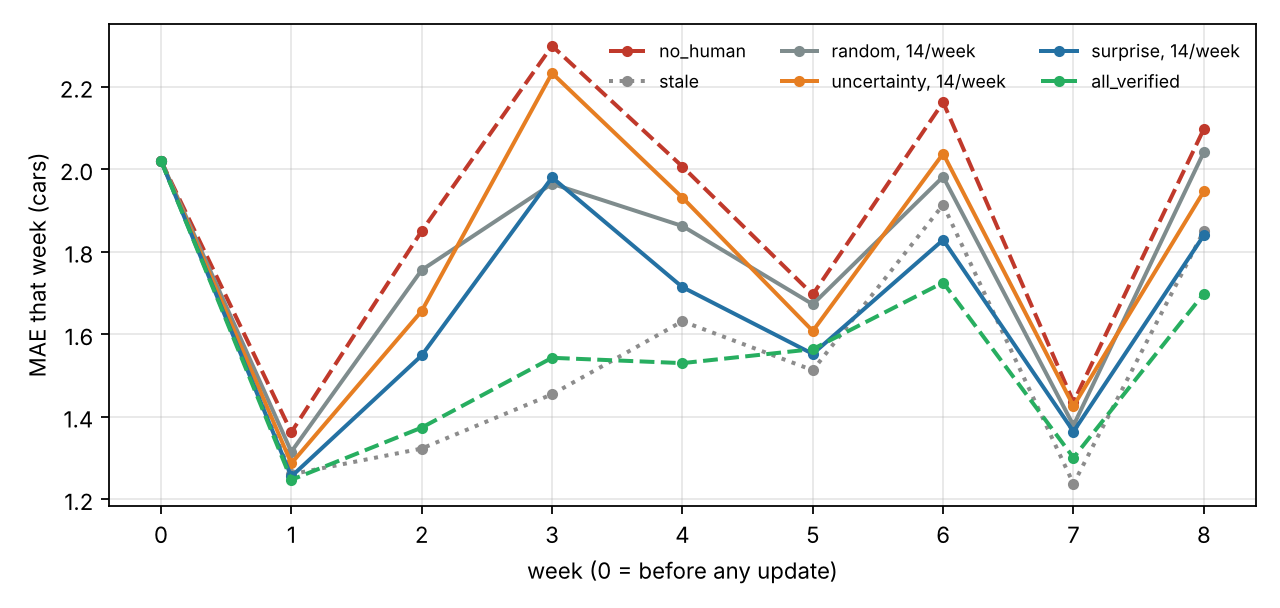
\includegraphics[width=0.85\textwidth]{figures/mae_per_week_jpl.png}
\caption{Weekly MAE under the \emph{scheduled} policy (previous design), with 14 operator checks per week for the
three query strategies. Retraining on unchecked data (\texttt{no\_human}) is worse than never retraining
(\texttt{stale}) in every week, which motivated the champion--challenger gate. The same plot for the selected
technique: \run.}
\end{figure}

\textbf{Efficiency during continual updates.}

\begin{table}[H]
\centering\small
\begin{tabular}{@{}lc@{}}
\toprule
Metric & Value \\
\midrule
Challenger training time (DLinear + Ridge + stacking + CQR, CPU) & 7.2--8.4\,s \\
Training time, 6-month buffer vs all data since 2019 & 6.6\,s vs 20\,s \\
Inference latency per forecast (stacking, p50) & 0.31\,ms (unchanged) \\
Extra inference during a shadow week & one 0.31\,ms forecast per 15-minute step \\
Daily query selection (digest) & $<5$\,ms \\
Peak memory during an update (RSS) & \run \\
Artifact size per version & 320\,KiB (weights) + \run \\
\bottomrule
\end{tabular}
\end{table}

% =====================================================================
\section*{2.1 When and Why Humans Intervene}

In our system the true occupancy arrives on its own 4 hours after each forecast, so humans are not needed to provide
answers. They are needed because \textbf{the telemetry itself can be wrong} in ways that look normal (Section 1.4).
A grid operator intervenes in three situations:
\begin{itemize}
  \item \textbf{Labeling suspicious predictions (daily digest).} Every evening the operator checks the two forecasts
  that most surprised the model (Section 2.3) and decides, using the chargers' own session logs, the parking camera or
  a site visit, whether the telemetry was a real event (a campus event, a busy day) or a sensor fault.
  \item \textbf{Validating drift and anomaly alerts (linked to M3 monitoring).} When a retraining trigger fires, the
  operator confirms whether it reflects a lasting change (new chargers, new schedule) or a data incident (such as the
  six-day JPL outage of July 2021 found by our data-quality monitor). A challenger is never trained on an outage.
  \item \textbf{Approving model outputs (promotion).} The operator signs off the shadow report before a challenger
  replaces the champion.
\end{itemize}

% =====================================================================
\section*{2.2 How Human Input is Incorporated}

\begin{itemize}
  \item \textbf{As new labeled data for continual updates.} A correction replaces the faulty telemetry of the checked
  4-hour block in the label store; the next challenger trains on the corrected values, verified windows get a
  $2\times$ sample weight and never expire from the buffer.
  \item \textbf{As gating (accept/reject) logic.} Verified windows form part of the trusted data on which the challenger
  is compared with the champion, and a challenger cannot be promoted without the operator's sign-off.
  \item \textbf{As constraints or rules.} Fault patterns the operator keeps confirming become automatic rules (for
  example, a value repeated exactly for more than 2 hours of daytime is flagged as a frozen gateway), so routine
  faults stop needing a human.
  \item \textbf{As feedback for active learning.} Each verdict (\emph{corrected}, \emph{confirmed real event},
  \emph{missed}) is logged; a growing share of confirmed real events is itself a sign of drift and feeds the
  confirmed-change trigger.
\end{itemize}

% =====================================================================
\section*{2.3 Active Learning Strategy}

\textbf{Query strategy: nonconformity (surprise) sampling with temporal diversity.} For each forecast whose 4 hours
ended today we know the interval $[\hat y_{10}, \hat y_{90}]$ published in the morning and the telemetry $y$ that
came in. The query score is the Split-CQR nonconformity score of the received telemetry:
\[
\text{surprise} = \frac{1}{16}\sum_{h=1}^{16} \max\!\left(\hat y_{10,h} - y_h,\; y_h - \hat y_{90,h},\; 0\right).
\]
The operator checks the forecasts with the highest surprise, skipping any forecast whose 4-hour block overlaps one
already selected (consecutive forecasts 15 minutes apart cover almost the same hours, so without this rule two checks
would look at the same fault). We compared it with classic uncertainty sampling on the interval width
$W=\hat y_{90}-\hat y_{10}$ and with random sampling. On the first two drifted weeks, surprise separates faulty from
healthy windows much better than width (AUC 0.83 vs 0.62): a wide interval means the model is unsure, not that the
data is wrong.

\textbf{Sampling frequency and update loop.} A daily digest of 2 forecasts per evening (14 per week, about
0.7 operator-hours per week at 3 minutes per check). Corrections are written to the label store immediately and used
by the next challenger and by the next shadow evaluation.

\textbf{Interaction with continual learning.}
(1) Corrected windows clean the replay buffer before a challenger is trained, so faults do not reach the model.
(2) Verified windows are part of the trusted data that decides the champion--challenger comparison.
(3) Forecasts that are surprising but not yet checked are quarantined (weight 0) from training.
(4) A rising share of confirmed real events in the digest feeds the confirmed-change trigger.

\begin{figure}[H]
\centering
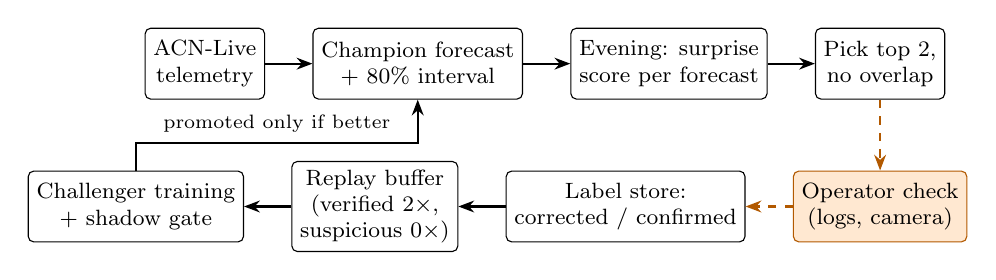
\begin{tikzpicture}[node distance=0.55cm and 0.6cm]
  \node[box] (tel) {ACN-Live\\telemetry};
  \node[box, right=of tel] (fc) {Champion forecast\\+ 80\% interval};
  \node[box, right=of fc] (sc) {Evening: surprise\\score per forecast};
  \node[box, right=of sc] (pick) {Pick top 2,\\no overlap};
  \node[hum, below=0.9cm of pick] (op) {Operator check\\(logs, camera)};
  \node[box, left=of op] (ls) {Label store:\\corrected / confirmed};
  \node[box, left=of ls] (buf) {Replay buffer\\(verified $2\times$,\\suspicious $0\times$)};
  \node[box, left=of buf] (ch) {Challenger training\\+ shadow gate};
  \draw[arr] (tel) -- (fc);
  \draw[arr] (fc) -- (sc);
  \draw[arr] (sc) -- (pick);
  \draw[harr] (pick) -- (op);
  \draw[harr] (op) -- (ls);
  \draw[arr] (ls) -- (buf);
  \draw[arr] (buf) -- (ch);
  \draw[arr] (ch.north) -- ++(0,0.35) -| node[pos=0.25, above, font=\scriptsize] {promoted only if better} (fc.south);
\end{tikzpicture}
\caption{Active learning loop. Orange = human step.}
\end{figure}

% =====================================================================
\section*{2.4 Human-in-the-Loop Simulation}

\textbf{Setup.} Same drift and fault scenario as Section 1.4 (JPL, 8 weeks, 3 seeds). Human annotation is simulated
with synthetic labels: the operator looks up the true telemetry for the checked 4-hour block and enters it, but misses a
fault 5\% of the time. Each week a challenger is trained on the buffer curated by each strategy and scored on the
following week of true data; this isolates the value of the labels for an update. We compare 3, 7 and 14 checks per
week with three query strategies, between two references: no human (0\%) and every window verified (100\%).

\begin{figure}[H]
\centering
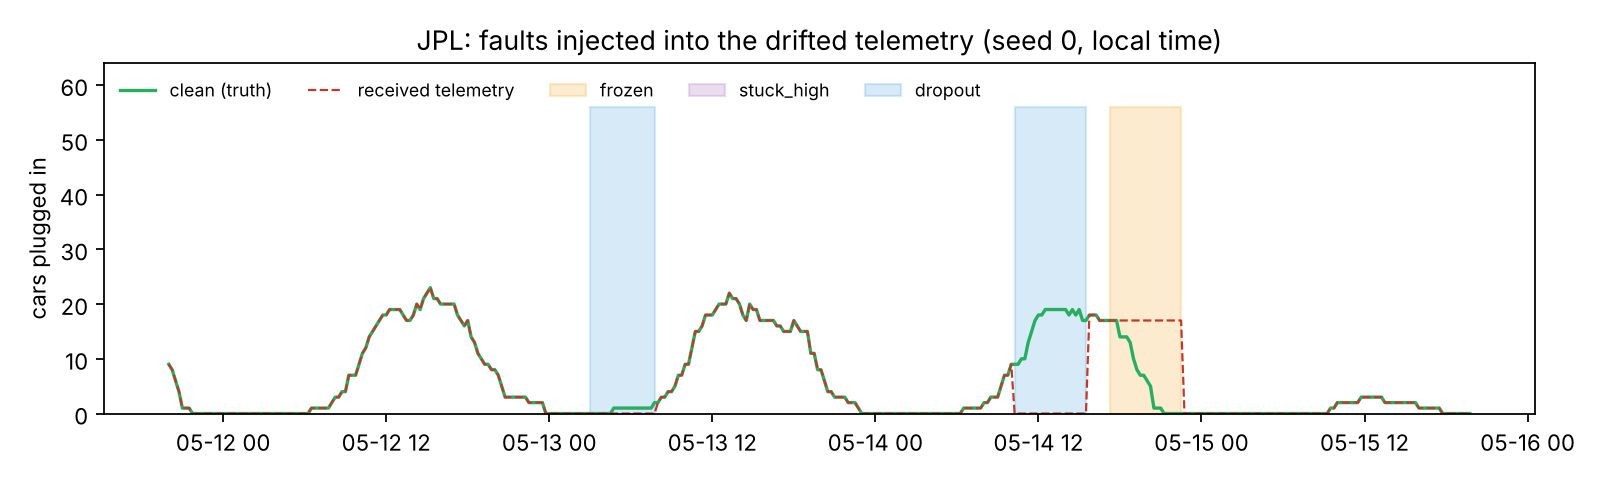
\includegraphics[width=0.8\textwidth]{figures/fault_example.png}
\caption{Simulated faults (seed 0): true occupancy (green) vs received telemetry (red).}
\end{figure}

\begin{table}[H]
\centering\small
\caption{Challenger quality by query strategy and budget (weeks 1--8, mean of 3 seeds). Damage removed: 0\% = no
human (MAE 1.86), 100\% = everything verified (MAE 1.50).}
\begin{tabular}{@{}lccccc@{}}
\toprule
Strategy, checks/week & MAE & Damage removed & Faults fixed & Checks finding a fault & Operator h/week \\
\midrule
random, 3        & 1.81 & 14\% & 7\%  & 19\% & 0.15 \\
uncertainty, 3   & 1.83 &  9\% & 7\%  & 19\% & 0.15 \\
surprise, 3      & 1.85 &  4\% & 7\%  & 10\% & 0.15 \\
random, 7        & 1.78 & 22\% & 14\% & 14\% & 0.35 \\
uncertainty, 7   & 1.83 & 10\% & 13\% & 15\% & 0.35 \\
surprise, 7      & 1.80 & 18\% & 21\% & 17\% & 0.35 \\
random, 14       & 1.75 & 32\% & 31\% & 14\% & 0.70 \\
uncertainty, 14  & 1.77 & 27\% & 18\% & 14\% & 0.70 \\
\textbf{surprise, 14} & \textbf{1.64} & \textbf{62\%} & \textbf{49\%} & \textbf{18\%} & \textbf{0.70} \\
everything verified & 1.50 & 100\% & 100\% & -- & 33.5 \\
\bottomrule
\end{tabular}
\end{table}

\begin{figure}[H]
\centering
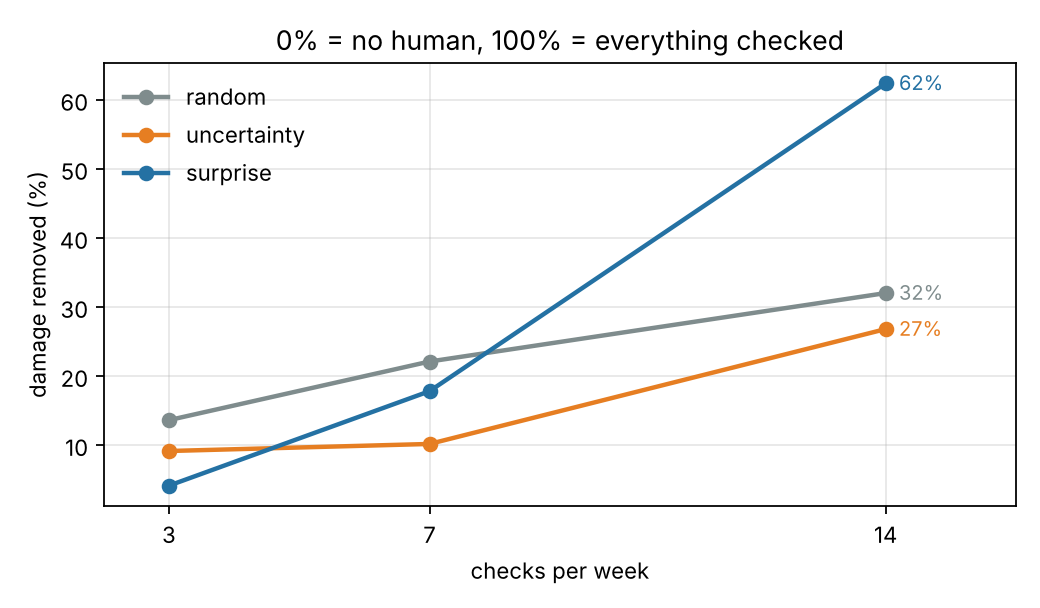
\includegraphics[width=0.6\textwidth]{figures/damage_removed_jpl.png}
\caption{Share of the damage removed by each query strategy as the budget grows.}
\end{figure}

\textbf{Performance across cycles.} With 14 checks per week, surprise sampling removes 62\% of the damage caused by
faulty telemetry, against 32\% for random and 27\% for width-based uncertainty sampling. It beats random with all 3
seeds (MAE 1.53 vs 1.64, 1.77 vs 1.89, 1.61 vs 1.71) and in 19 of the 24 seed-weeks. With 3 or 7 checks per week no
strategy beats random (differences within the seed-to-seed spread of $\pm$0.14--0.19 cars): one check per evening
cannot keep up with about 4 fault events per week.

\textbf{Efficiency.}
\begin{itemize}
  \item \textbf{Labeling burden:} 0.7 operator-hours per week remove 62\% of the damage, against 33.5 hours to
  verify everything (2\% of the effort).
  \item \textbf{Stability of continual updates:} the weekly MAE varies less between seeds when more faults are fixed:
  spread 0.33 with no human, 0.20--0.23 for random and width at 14 checks/week, 0.14 for surprise, 0.01 with
  everything verified.
  \item \textbf{Latency impact:} selecting the daily queries takes under 5\,ms; challenger training (7--8\,s) and the
  forecast latency are unchanged by the human loop.
  \item \textbf{Width-based sampling wastes checks:} with the same 14 checks per week it covered only 19\% of the new
  data (33\% for surprise), because the widest intervals of a day are consecutive forecasts over the same hours.
\end{itemize}
\textbf{With the champion--challenger gate} (selected technique): promotions accepted \run, rejected \run, final MAE
\run.

% =====================================================================
\section*{3.1 Complete System Diagram}

\begin{figure}[H]
\centering
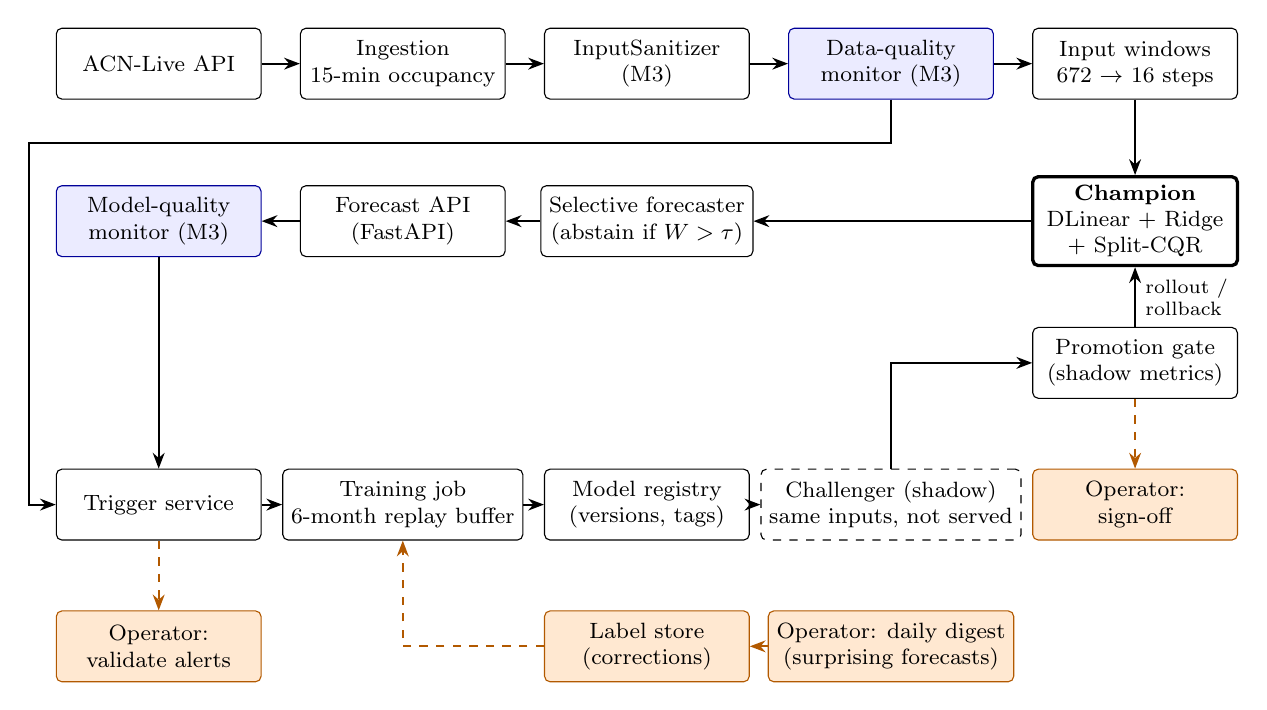
\begin{tikzpicture}[every node/.style={font=\footnotesize}, box/.append style={minimum width=2.6cm}]
  % columns 1.3, 4.4, 7.5, 10.6, 13.7 ; rows 0, -2, -3.8, -5.6, -7.4
  \node[box] (api) at (1.3,0) {ACN-Live API};
  \node[box] (ing) at (4.4,0) {Ingestion\\15-min occupancy};
  \node[box] (san) at (7.5,0) {InputSanitizer\\(M3)};
  \node[mon] (dq)  at (10.6,0) {Data-quality\\monitor (M3)};
  \node[box] (win) at (13.7,0) {Input windows\\672 $\to$ 16 steps};
  \node[mon] (mq)  at (1.3,-2) {Model-quality\\monitor (M3)};
  \node[box] (out) at (4.4,-2) {Forecast API\\(FastAPI)};
  \node[box] (sel) at (7.5,-2) {Selective forecaster\\(abstain if $W>\tau$)};
  \node[box, very thick] (champ) at (13.7,-2) {\textbf{Champion}\\DLinear + Ridge\\+ Split-CQR};
  \node[box] (gate) at (13.7,-3.8) {Promotion gate\\(shadow metrics)};
  \node[box] (trig) at (1.3,-5.6) {Trigger service};
  \node[box] (train) at (4.4,-5.6) {Training job\\6-month replay buffer};
  \node[box] (reg) at (7.5,-5.6) {Model registry\\(versions, tags)};
  \node[box, dashed] (chal) at (10.6,-5.6) {Challenger (shadow)\\same inputs, not served};
  \node[hum] (sign) at (13.7,-5.6) {Operator:\\sign-off};
  \node[hum] (val) at (1.3,-7.4) {Operator:\\validate alerts};
  \node[hum] (ls)  at (7.5,-7.4) {Label store\\(corrections)};
  \node[hum] (dig) at (10.6,-7.4) {Operator: daily digest\\(surprising forecasts)};

  \draw[arr] (api) -- (ing);
  \draw[arr] (ing) -- (san);
  \draw[arr] (san) -- (dq);
  \draw[arr] (dq) -- (win);
  \draw[arr] (win) -- (champ);
  \draw[arr] (champ) -- (sel);
  \draw[arr] (sel) -- (out);
  \draw[arr] (out) -- (mq);
  \draw[arr] (mq) -- (trig);
  \draw[arr] (dq.south) -- ++(0,-0.55) -| (-0.35,-5.6) -- (trig.west);
  \draw[arr] (trig) -- (train);
  \draw[arr] (train) -- (reg);
  \draw[arr] (reg) -- (chal);
  \draw[arr] (chal.north) |- (gate.west);
  \draw[arr] (gate) -- node[right, font=\scriptsize, align=left] {rollout /\\rollback} (champ);
  \draw[harr] (gate) -- (sign);
  \draw[harr] (trig) -- (val);
  \draw[harr] (dig) -- (ls);
  \draw[harr] (ls.west) -| (train.south);
\end{tikzpicture}
\caption{Complete system. Blue = Milestone 3 monitors (now also retraining triggers), orange = human interactions,
dashed = shadow path. Every challenger is an immutable registry version; the gate promotes it (rollout) or the
previous champion is restored (rollback), each with its own calibration.}
\end{figure}

% =====================================================================
\section*{3.2 Updates to Failure Modes and Monitoring}

\begin{table}[H]
\centering\small
\begin{tabularx}{\textwidth}{@{}p{3.6cm}YY@{}}
\toprule
New failure mode & Detection & Mitigation \\
\midrule
Challenger trained on faulty telemetry & shadow MAE worse than champion & gate rejects it; quarantine of unverified suspicious windows \\
Biased evaluation set (only unusual windows are verified) & share of verified vs unflagged windows in the trusted set & trusted set = verified \emph{and} unflagged windows \\
Trigger storm (flapping alerts) & triggers per week & one challenger at a time, 7-day cooldown \\
Champion ages silently (no trigger fires) & days since last promotion & age trigger at 8 weeks \\
Operator overload or mistakes & digest backlog, verdict mix & cap of 2 checks per evening; sign-off reviews the shadow report \\
Feedback loop (the model decides what gets labeled) & share of confirmed real events & reserve some checks for random windows to keep an unbiased error estimate \\
Wrong rollout or broken artifact & post-promotion MAE ratio (M3 rule) & automatic rollback to the previous champion and its calibration \\
\bottomrule
\end{tabularx}
\end{table}

\textbf{New monitoring signals.} Champion vs challenger MAE and coverage during shadow weeks; promotion and rejection
log with trigger reasons; digest backlog and verdict mix (\% corrected, \% real events, \% missed); share of the
buffer that is verified or quarantined; time since the last promotion. The Milestone 3 SLOs (MAE ratio $\le 0.80$,
coverage 75--85\%, p95 latency $\le 50$\,ms, freshness $\le 2$\,min) are unchanged.

% =====================================================================
\section*{3.3 Impact of Continual Learning and HITL}

\begin{itemize}
  \item \textbf{Latency.} Inference is unchanged (0.31\,ms p50 per forecast). A shadow week adds one extra forecast per
  15-minute step, off the serving path. The update cycle is slower than a weekly schedule: at least one week of shadow
  evaluation after a trigger, while coverage problems are fixed the same day by recalibration.
  \item \textbf{Accuracy and robustness.} The gate prevents regressions from updates (unchecked scheduled retraining
  cost +24\% MAE in our simulation). Curated labels make challengers better: surprise sampling at 14 checks per week
  removes 62\% of the damage caused by faulty telemetry.
  \item \textbf{Interpretability and trust.} Every deployed model has a traceable reason (trigger), evidence (shadow
  metrics on trusted data) and a human approval. The verdict log explains data problems in plain terms (frozen
  gateway, outage, real event).
  \item \textbf{Resource utilization.} CPU only; 7--8\,s per challenger; 676\,MiB RSS; 320\,KiB of weights per
  version. Human time: about 0.7 hours per week for the digest plus a few minutes per promotion, against 33.5 hours to
  check everything.
\end{itemize}

% =====================================================================
\section*{3.4 System Summary}

\begin{table}[H]
\centering\small
\caption{Key results across the project (JPL unless noted).}
\begin{tabularx}{\textwidth}{@{}lY@{}}
\toprule
Milestone & Key result \\
\midrule
M1: problem and data & ACN-Data (Caltech, JPL), plug occupancy at 15 minutes, 4-hour horizon; \fillin{dataset size and period} \\
M2: model selection & DLinear chosen (CPU FP32): MAE 1.844 (Caltech 0.904), 80\% coverage 80.0\% after Split-CQR; 64{,}626 parameters, 0.14\,ms p50 \\
M3: robustness and monitoring & stacking DLinear + Ridge MAE 1.775; corrupted telemetry crashes the model without the sanitizer (NaN), MAE 1.750 with it; Time-of-Use drift 1.775 $\to$ 1.899, recovered 1.773 after retraining; abstention on 10\% widest intervals: MAE 1.562; data- and model-quality monitors with alert, rollback and recalibration policies \\
M4: continual learning + HITL & scheduled retraining on unchecked data: +24\% MAE; surprise sampling removes 62\% of that damage with 0.7 operator-hours/week; champion--challenger: \run \\
\bottomrule
\end{tabularx}
\end{table}

\begin{table}[H]
\centering\small
\caption{Final performance (MAE in cars / calibrated 80\% coverage).}
\begin{tabular}{@{}lcc@{}}
\toprule
Condition & JPL & Caltech \\
\midrule
Clean test set, stacking (M3) & 1.775 / 81.5\% & 0.927 / 76.6\% \\
Corrupted telemetry + sanitizer (M3) & 1.750 / 78.0\% & 0.765 / 76.0\% \\
Time-of-Use drift, not updated (M3) & 1.899 / 80.3\% & 0.949 / 77.7\% \\
Drift + sensor faults, after CL + HITL (M4, 8-week replay) & \run & not run \\
\bottomrule
\end{tabular}
\end{table}

\begin{table}[H]
\centering\small
\caption{Final efficiency (CPU, no GPU; JPL).}
\begin{tabular}{@{}lc@{}}
\toprule
Metric & Value \\
\midrule
Training time, full history / 6-month buffer & 20\,s / 6.6\,s \\
Update time (one challenger) & 7.2--8.4\,s \\
Inference latency, single forecast p50 / p90 & 0.31\,ms / 0.33\,ms \\
Inference latency, batch p50 & 1.61\,ms \\
Throughput & 39{,}700 samples/s \\
Model size & 76{,}674 parameters, 320\,KiB \\
Memory (RSS) / VRAM & 676\,MiB / 0 (CPU) \\
\bottomrule
\end{tabular}
\end{table}

\textbf{Reflection.}
\begin{itemize}
  \item \textbf{Strengths.} A light, fast model (seconds to retrain, sub-millisecond inference) with calibrated
  intervals; monitors that catch data and model problems; updates that cannot make the system worse; and a human loop
  that targets the one thing the model cannot know: whether the telemetry is real.
  \item \textbf{Limitations.} The Milestone 4 experiments use one site (JPL), simulated faults and a simulated operator,
  and 3 seeds. The injected faults land far from the expected range, which favours surprise sampling; a small constant
  bias would be harder to catch. The gate needs enough trusted data in a shadow week, and the system reacts to real
  changes only after a week of shadow evaluation. Holidays and campus events remain the main forecasting errors.
  \item \textbf{Future improvements.} A daily correction layer on top of the champion (bias correction per hour and
  adaptive conformal intervals) for faster small adjustments; automatic rules for obvious faults (frozen values);
  holiday and academic-calendar features; a real operator study; repeating the experiments on Caltech.
\end{itemize}

\end{document}
